\chapter{Resultados del estudio de base}
\label{cap:resultados}

Este capítulo presenta los resultados del estudio de base realizado en \emph{vision}.
El registro contiene 133 identificadores de corrida, tomando la última
entrada de cada uno: 119 completadas (96 de detección y 23 de
spoiling) y 14 con error. Como no todas usan los mismos datos y protocolos,
las tablas y figuras muestran solo comparaciones compatibles. El registro
completo y las respuestas de cada ejemplo pueden consultarse en Power BI.

\section{Detección: calidad y cómputo}

La línea base de TF-IDF con unigramas, bigramas y trigramas, más un SVM
lineal, obtuvo F1 de clickbait 0,6646 en los 700 ejemplos de desarrollo.
Una ejecución anterior sobre los 700 ejemplos de prueba obtuvo 0,6165.
La prevalencia de clickbait baja de 203/700 en desarrollo a 167/700 en
prueba; por ello, esta diferencia de F1 no debe atribuirse por sí sola
a una pérdida de generalización del clasificador.
Una variante de RoBERTa-BNE con ponderación de clases alcanzó 0,8900 en
desarrollo y aún no se evaluó en prueba. El detector publicado de dcere
figura con 0,9127 en el registro, pero se ajustó con datos de desarrollo.
Por ese motivo no se incluye en la comparación sobre ese conjunto.

\begin{table}[htbp]
\centering
\caption{Resultados de detección. F1 corresponde a la clase clickbait y OOF
a predicciones fuera de fold. Los resultados de 700 y 3.500 ejemplos se
obtuvieron con protocolos distintos.}
\label{tab:det-resultados}
\begin{tabular}{p{7.2cm}rcc}
\toprule
Configuración & $n$ & Protocolo & F1 \\
\midrule
TF-IDF + SVM lineal & 700 & dev & 0,6646 \\
RoBERTa-BNE con clases ponderadas & 700 & dev & 0,8900 \\
D10b, solo texto (T) & 3.500 & OOF CV5 & 0,8500 \\
D10b, texto e imagen (TI) & 3.500 & OOF CV5 & 0,8523 \\
D11a, fusión MLP fija (TI) & 3.500 & OOF CV5 & 0,8455 \\
\bottomrule
\end{tabular}
\end{table}

Las figuras~\ref{fig:pareto-det} y~\ref{fig:pareto-spo} comparan calidad y
cómputo en desarrollo para 54 corridas de detección y 16 de spoiling con
FLOPs estimados. Los puntos del frente no están dominados por otras
configuraciones de este registro. Las corridas OOF de visión y los servicios
por API quedan fuera de estos gráficos porque usan otro protocolo o no
tienen FLOPs comparables. En detección, pasar de clasificadores léxicos a
RoBERTa-BNE mejora la calidad, pero aumenta el cómputo en varios órdenes
de magnitud. El frente podría cambiar al probar otras configuraciones.

\begin{figure}[htbp]
\centering
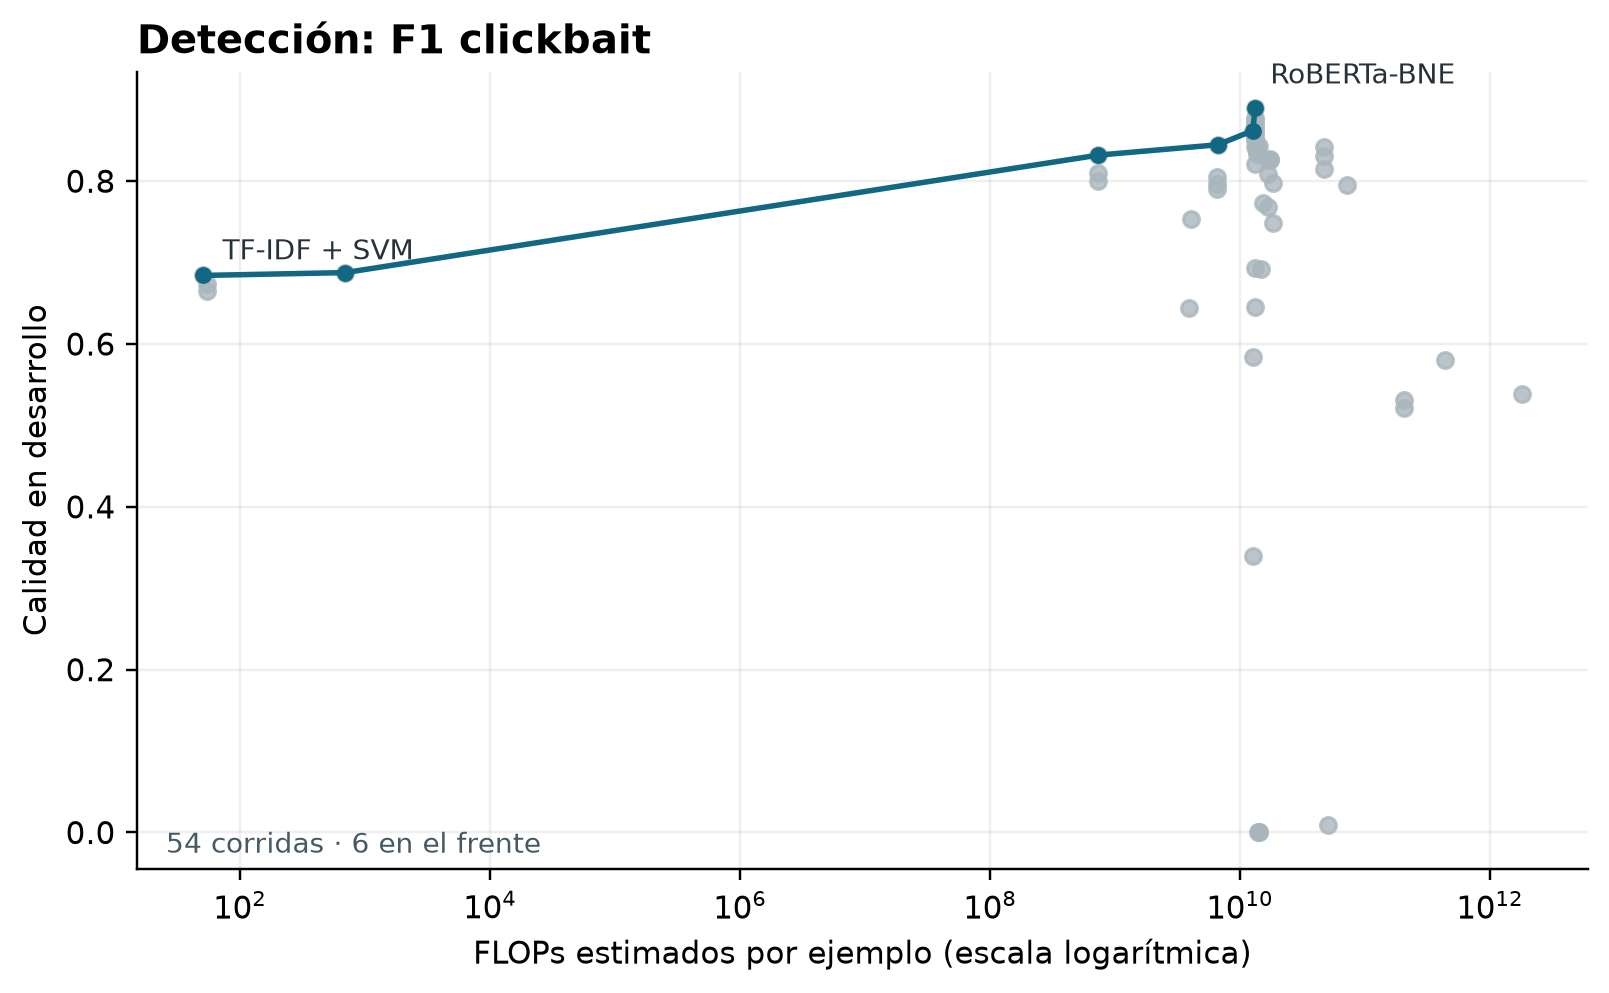
\includegraphics[width=\textwidth]{figuras/frente_detection.png}
\caption{Calidad y cómputo de detección en desarrollo. Los FLOPs se
estiman por ejemplo; la línea une los puntos no dominados.}
\label{fig:pareto-det}
\end{figure}

\begin{figure}[htbp]
\centering
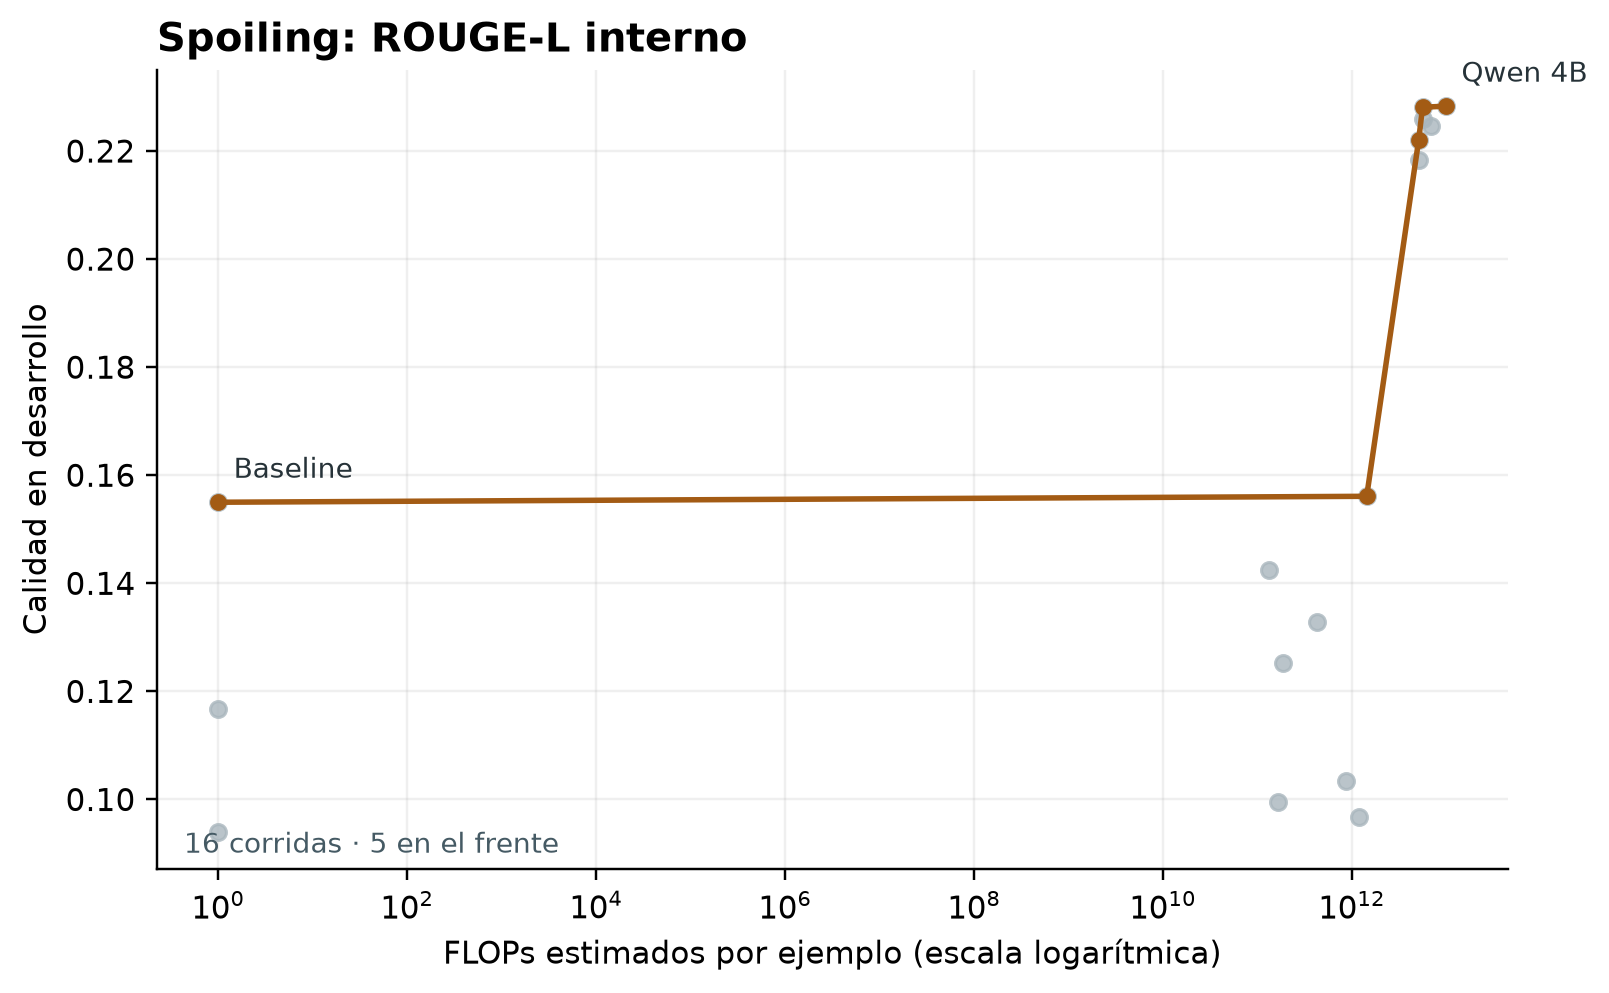
\includegraphics[width=\textwidth]{figuras/frente_spoiling.png}
\caption{Calidad y cómputo de spoiling en desarrollo. ROUGE-L procede de
la implementación local. Los servicios por API no tienen FLOPs comparables.}
\label{fig:pareto-spo}
\end{figure}

\section{Spoiling: calidad interna y salidas}

La réplica de la heurística oficial obtuvo ROUGE-L local 0,1550 y
BERTScore 0,6533 en los 100 ejemplos de desarrollo. En prueba, su BERTScore
fue 0,6637, cercano al 0,661 informado por la tarea compartida. En
desarrollo, Qwen 3.5 4B obtuvo ROUGE-L 0,2283 y BERTScore 0,6996.
GPT-5.6 Luna alcanzó 0,2884 y 0,7273 sin imagen; con imagen, 0,3151
y 0,7350. La diferencia pareada de ROUGE-L fue $+0,0267$, con IC del
95\,\% $[-0,0073;0,0641]$, que incluye cero. Estas corridas generativas
aún no tienen una evaluación final en prueba. En las condiciones de estas
ejecuciones, Luna costó aproximadamente USD 0,327 por 1.000 ejemplos sin
imagen y USD 0,636 con imagen. Ese costo no es comparable con los FLOPs
de los modelos locales.

\section{Aporte de la imagen}

Las figuras~\ref{fig:vision-det} y~\ref{fig:vision-spo} muestran las
comparaciones pareadas entre T y TI. En D10a, DeiT+Beto pasó de F1
0,6960 a 0,6718 al añadir la imagen: una diferencia de $-0,0242$,
con IC del 95\,\% $[-0,0444;-0,0055]$ sobre 3.500 predicciones OOF.
La variante con SigLIP2 también bajó $-0,0254$
($[-0,0499;-0,0002]$). Estos descensos corresponden a las
arquitecturas y entradas probadas.

D10b, con MLP residual, pasó de F1 0,8500 (T) a 0,8523 (TI):
una diferencia de $+0,0023$, con IC del 95\,\% $[-0,0047;0,0098]$.
Las cuatro comparaciones D11, realizadas con una semilla, tampoco
mostraron una mejora concluyente. Las diferencias fueron $+0,0009$ para
MLP \emph{fixed}, $-0,0005$ para atención \emph{fixed}, $-0,0035$ para
MLP \emph{joint} y $+0,0023$ para atención \emph{joint}; todos los
intervalos incluyeron cero. Con \emph{fixed}, las predicciones de los
555 ejemplos sin imagen son idénticas a las del modelo textual. Con
\emph{joint}, el entrenamiento también cambia algunas de esas
predicciones, de modo que la diferencia no refleja solo el uso de la imagen.

En spoiling, las tres comparaciones de Gemma 4 E2B con imagen o pie de
foto tuvieron diferencias de ROUGE-L entre $+0,0026$ y $+0,0061$.
LFM 2.5 VL registró $-0,0067$. Todos los intervalos del 95\,\%
incluyeron cero. En conjunto, estos experimentos no muestran una mejora
visual general en las configuraciones estudiadas y señalan qué casos
merecen una evaluación más controlada.

\begin{figure}[htbp]
\centering
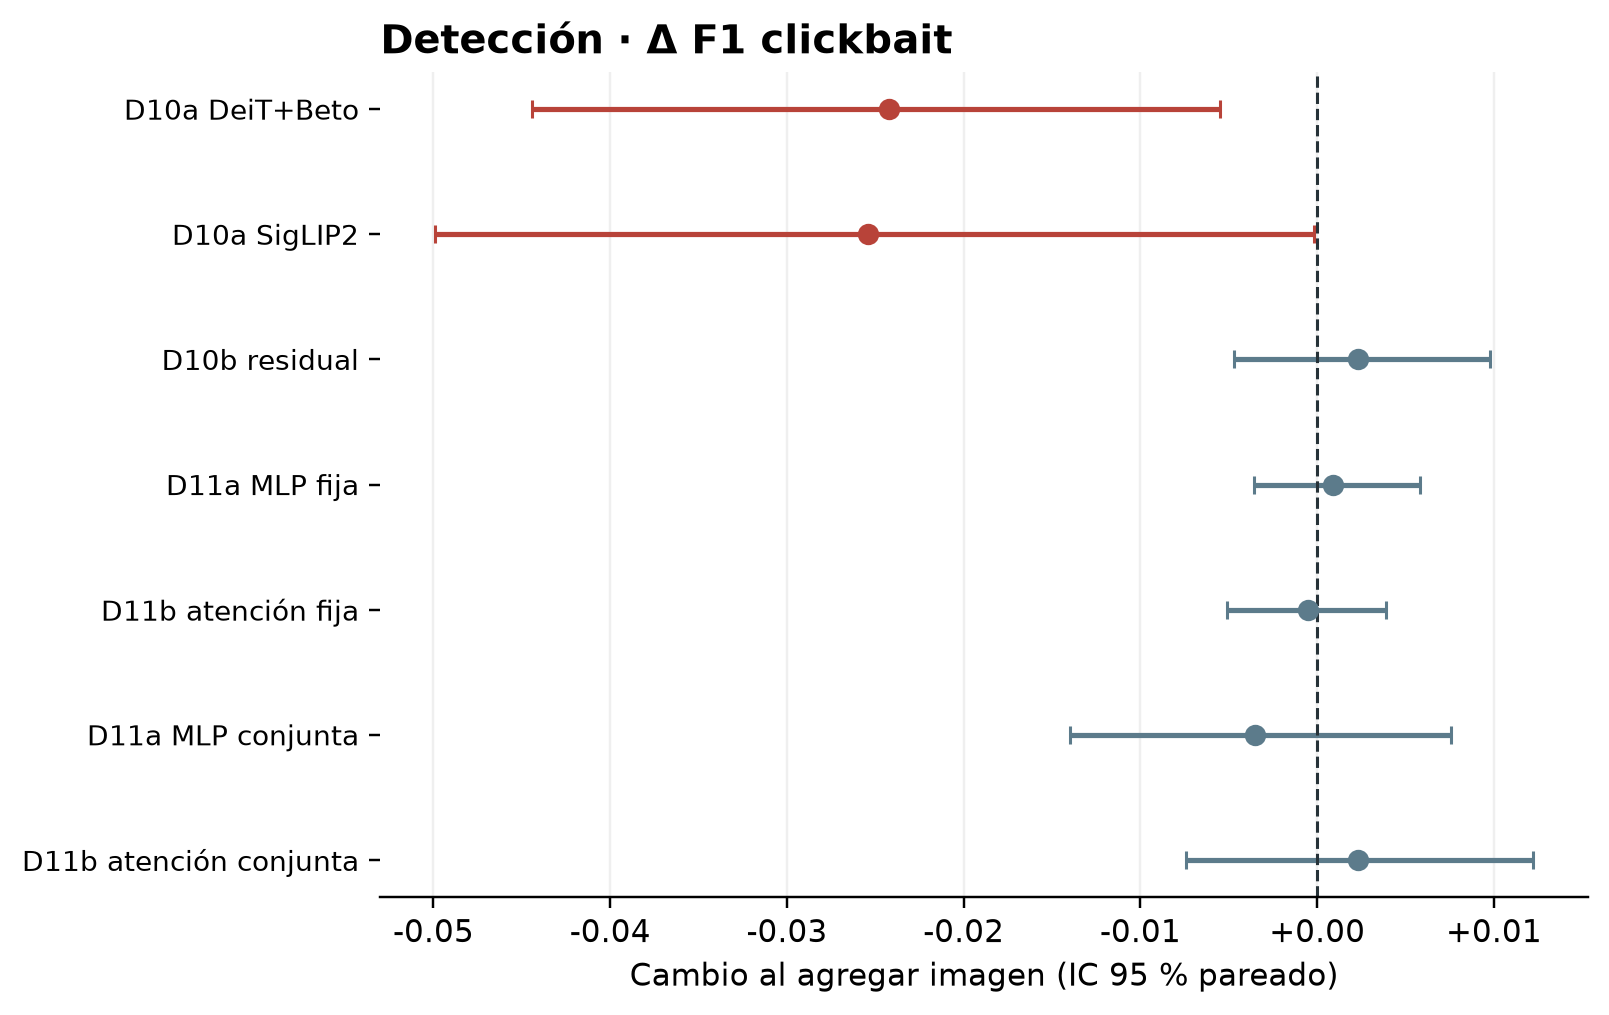
\includegraphics[width=\textwidth]{figuras/ablacion_detection.png}
\caption{Diferencia pareada de F1 al añadir imagen en detección. Se
muestran todos los ejemplos; D10 y D11 usan predicciones OOF.}
\label{fig:vision-det}
\end{figure}

\begin{figure}[htbp]
\centering
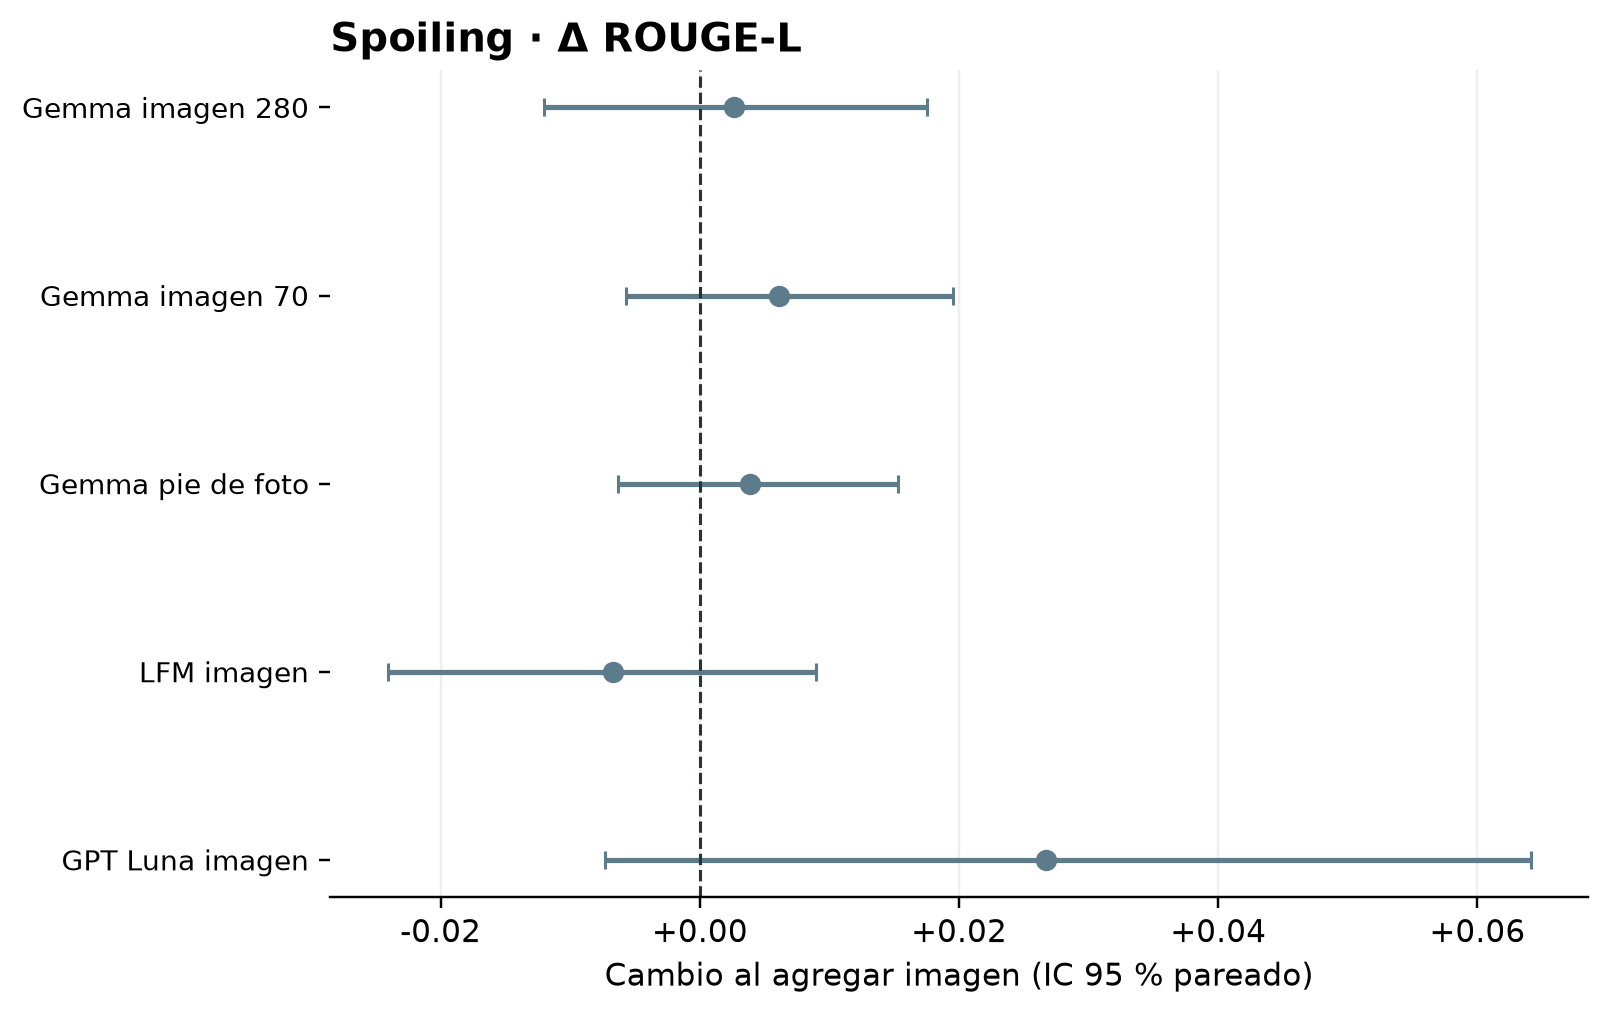
\includegraphics[width=\textwidth]{figuras/ablacion_spoiling.png}
\caption{Diferencia pareada de ROUGE-L local al añadir imagen o pie de
foto en spoiling, sobre todos los ejemplos de desarrollo.}
\label{fig:vision-spo}
\end{figure}

\section{Límites de interpretación}

Varias configuraciones se eligieron según su resultado en desarrollo, por
lo que las mejores cifras de ese conjunto pueden ser optimistas. Además,
la validación visual no separa duplicados, D11 se ejecutó con una sola
semilla y las imágenes recuperadas varían en disponibilidad y pertinencia.
Los intervalos calculados no recogen toda esa incertidumbre ni la selección
de familias de modelos después de inspeccionar desarrollo. El test oficial
de detección carece de imágenes y artículos, de modo que no es una prueba
final de los modelos multimodales. Las versiones
locales de ROUGE-L y BLEU tampoco reproducen la evaluación oficial de
spoiling. Por último, la comparación entre calidad y costo no incluye
la obtención de imágenes, el tiempo total de respuesta ni la valoración
humana de los spoilers. Los resultados deben leerse con estos límites
al establecer referencias para evaluar el marco de agentes.
